\begin{table}[tbp]
\centering\small
\caption{Matched-world organizational outcomes under a central record and daily updates.}
\label{tab:dynamic-results}
\begin{tabular}{lrrrrr}
\toprule
Policy & Work/member-day & Regret/guild-day & Mean days & P95 days & Unfinished \\
\midrule
Equal & 0.560 & 0.015 & 4.90 & 8.00 & 913 \\
Linear & 0.528 & 0.017 & 4.90 & 8.00 & 912 \\
DAMS & 0.532 & 0.016 & 4.90 & 8.00 & 913 \\
Performance tiers & 0.521 & 0.017 & 4.90 & 8.00 & 911 \\
Tenure tiers & 0.548 & 0.018 & 4.88 & 8.00 & 911 \\
\bottomrule
\end{tabular}
\par\smallskip\begin{minipage}{0.96\textwidth}\footnotesize Synthetic DAMS-ABM 0.1.0, source \texttt{3d67a62e6eb2}; 32 independent worlds, 120 members, four guilds, 60 days. Work and regret are model units. Delay is conditional on completed confirmations; unfinished records are the horizon stock. Entries are world means, not member-level independent samples.\end{minipage}
\end{table}
The prespecified primary contrast is 0.0036 [0.0031, 0.0041] generated work units per member-day for DAMS minus linear credit. The interval is the paired-world mean plus or minus 1.96 Monte Carlo standard errors. The fixed precision target is 0.01 and the substantive-effect threshold is 0.02 work units per member-day; neither criterion represents an externally estimated organizational effect.
\begin{figure}[tbp]
\centering
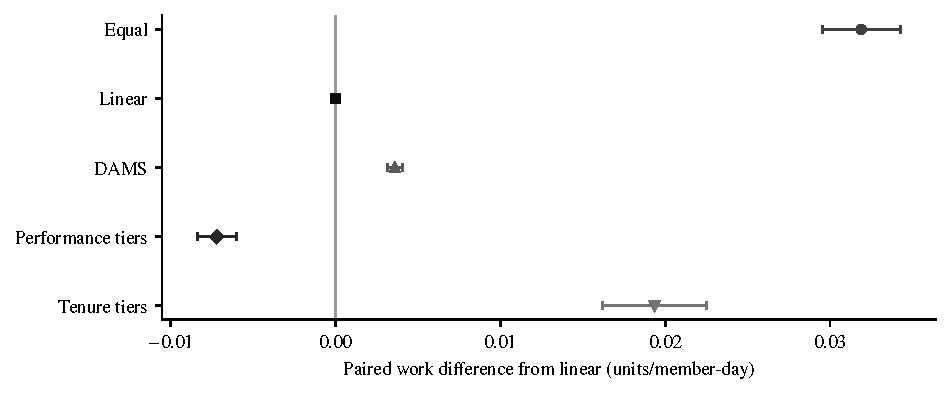
\includegraphics[width=\textwidth]{figures/results/allocation-effects.pdf}
\caption{Allocation effects relative to linear credit in 32 matched independent synthetic worlds. Symbols identify policies; bars are conditional 95\% normal Monte Carlo intervals. Equal baselines and the zero linear contrast are retained. Daily update, central record, 120 members and 60 days; source \texttt{3d67a62e6eb2}.}
\label{fig:allocation-effects}
\end{figure}
\begin{figure}[tbp]
\centering
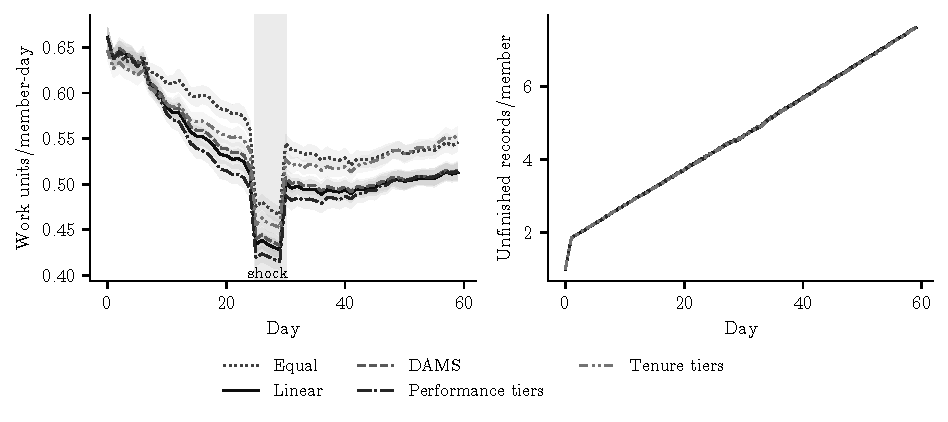
\includegraphics[width=\textwidth]{figures/results/governance-dynamics.pdf}
\caption{Daily generated work and unfinished review/settlement records in the same 32 worlds. Lines are world means and faint bands are pointwise 95\% Monte Carlo intervals; they are not trajectory prediction bands. The shaded site-0 shock lasts days 25--29. No smoothing is applied. The queue stock excludes appeals. DAMS-ABM 0.1.0, source \texttt{3d67a62e6eb2}.}
\label{fig:governance-dynamics}
\end{figure}
\begin{figure}[tbp]
\centering
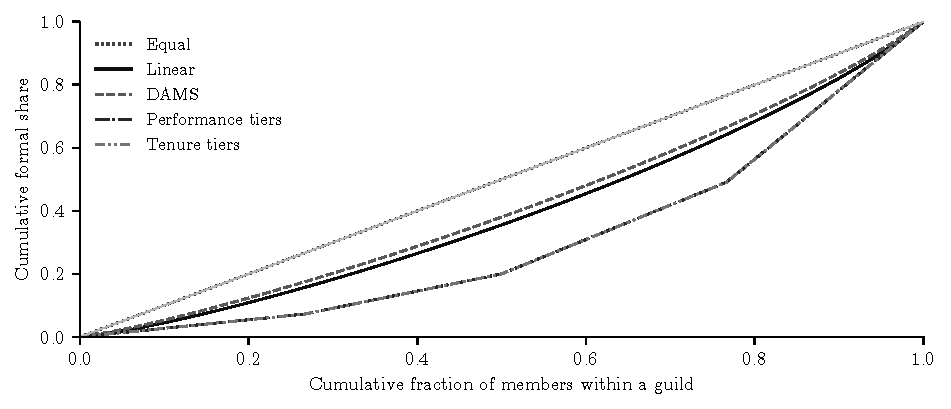
\includegraphics[width=\textwidth]{figures/results/formal-authority-distribution.pdf}
\caption{Final frozen formal-authority distributions for five policies, central record and daily updates. Lorenz curves are averaged across four 30-member guilds within each world and then over 32 independent worlds. Domain rights are not pooled into one organization-wide right. The diagonal indicates equal allocation; greater equality is not evidence of fairness, legitimacy or better decisions. Synthetic source \texttt{3d67a62e6eb2}.}
\label{fig:formal-authority-distribution}
\end{figure}
\begin{table}[tbp]
\centering\small
\caption{Same DAMS policy under three conditional evidence-process settings.}
\label{tab:ledger-stress}
\begin{tabular}{lrrrrr}
\toprule
Record & Work/member-day & Mean days & Unfinished & Review hours & Verify units \\
\midrule
Central & 0.532 & 4.90 & 913 & 637.2 & 0.0 \\
Witness & 0.538 & 10.48 & 2144 & 519.2 & 1038.4 \\
Consensus & 0.544 & 14.98 & 3120 & 424.8 & 2124.0 \\
\bottomrule
\end{tabular}
\par\smallskip\begin{minipage}{0.96\textwidth}\footnotesize 32 independent synthetic worlds per setting. Default cost multipliers and settlement delays are design assumptions, not measured database/log/consensus performance. Human review hours and extra verification units have different units. No monetary or total-cost equivalence is assumed.\end{minipage}
\end{table}
\begin{figure}[tbp]
\centering
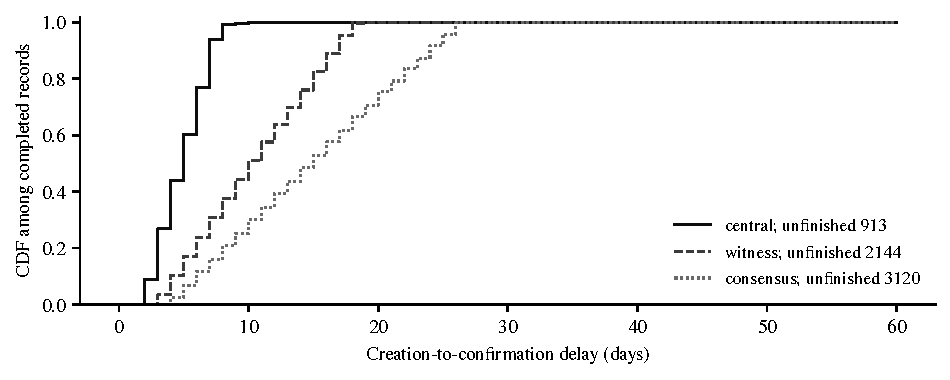
\includegraphics[width=\textwidth]{figures/results/confirmation-cdf.pdf}
\caption{Conditional delay distributions for DAMS under each evidence setting. Curves average the completed-record CDF of 32 independent worlds; legend values are mean unfinished horizon stocks. This is not a survival estimate for all submissions: incomplete records are excluded from each CDF and reported separately. Full integer-day steps are retained to day 60. Synthetic model source \texttt{3d67a62e6eb2}.}
\label{fig:confirmation-cdf}
\end{figure}
\begin{figure}[tbp]
\centering
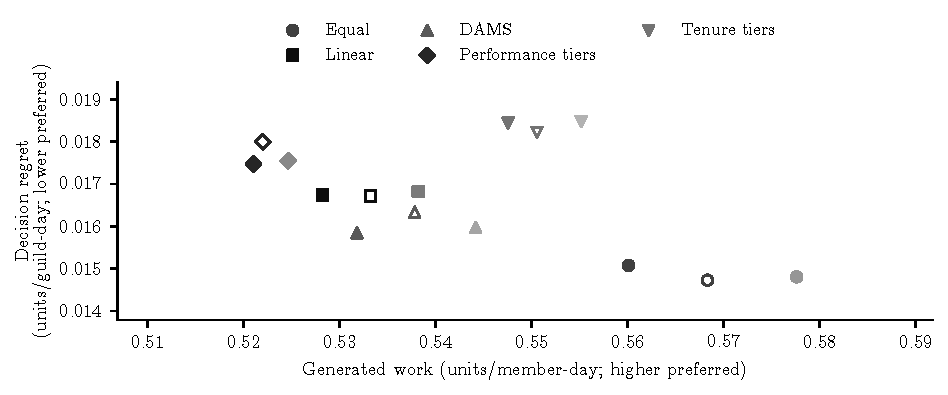
\includegraphics[width=\textwidth]{figures/results/outcome-tradeoffs.pdf}
\caption{Outcome-vector comparison for five policies and three record settings: 32-world means under daily update. Filled symbols denote central, hollow symbols witnessed and lighter filled symbols consensus assumptions. This diagram shows competing modeled objectives without converting them into welfare or money; uncertainty and paired effects are reported separately. A mean-position advantage does not establish universal Pareto dominance.}
\label{fig:outcome-tradeoffs}
\end{figure}
\begin{figure}[tbp]
\centering
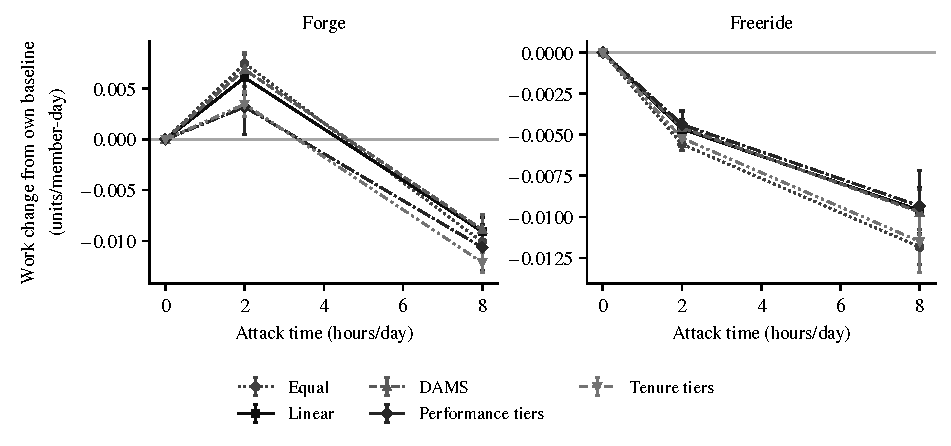
\includegraphics[width=\textwidth]{figures/results/attack-cost-effects.pdf}
\caption{Equal-time attack contrasts against each policy's own unattacked world. Eight independent worlds per cell, central record, 120 members, 60 days; fixed attacker cohort and ten active days. Points are sampled budgets, connected only as guides; bars are descriptive 95\% Monte Carlo intervals. Zero is the exact no-attack contrast, not an unexecuted missing cell. Forging raises observed claims and consumes time; free-riding also reduces real effort and help. These curves do not rank general security.}
\label{fig:attack-cost-effects}
\end{figure}
\begin{table}[tbp]
\centering\small
\caption{DAMS threat diagnostics under equal active-day time budgets.}
\label{tab:threat-diagnostics}
\begin{tabular}{lrrrrrr}
\toprule
Attack & \shortstack{Fraud\\committed} & \shortstack{Fraud initial\\rejections} & \shortstack{Honest review\\rejections} & \shortstack{Duplicate\\rejected} & Censored & \shortstack{Pending\\claims/appeals} \\
\midrule
None & 0.0 & 0.0 & 1449.2 & 0.0 & 0.0 & 914/4.6 \\
Forge & 229.5 & 401.0 & 1365.5 & 0.0 & 0.0 & 918/5.1 \\
Duplicate & 0.0 & 0.0 & 1666.0 & 405.8 & 0.0 & 1515/4.9 \\
Freeride & 0.0 & 0.0 & 1540.2 & 0.0 & 0.0 & 915/4.6 \\
Censor & 0.0 & 0.0 & 1585.2 & 0.0 & 43.9 & 872/5.1 \\
\bottomrule
\end{tabular}
\par\smallskip\begin{minipage}{0.96\textwidth}\footnotesize Eight matched independent worlds, central record, 120 members, 60 days, ten attack days at eight hour-equivalents/day. Entries are mean record counts; zero means no corresponding event, not missing data. Initial fraud rejections can later be appealed and committed; columns are nonexclusive events, not complementary detection rates. Honest review rejections count review events and can include duplicate submissions. Horizon stocks remain separate. Other policies and lower budgets are retained in the raw repository output.\end{minipage}
\end{table}
\begin{table}[tbp]
\centering\small
\caption{Equal-exposure and availability countercases for the same DAMS policy.}
\label{tab:record-countercases}
\begin{tabular}{lrrrr}
\toprule
Record & Equal exposure & Default exposure & Outage pending & Outage mean days \\
\midrule
Central & 41.9 & 41.9 & 912 & 4.91 \\
Witness & 41.9 & 21.2 & 2144 & 10.49 \\
Consensus & 41.9 & 0.0 & 3121 & 17.15 \\
\bottomrule
\end{tabular}
\par\smallskip\begin{minipage}{0.96\textwidth}\footnotesize Eight independent worlds per setting. The two censorship columns count censored records: equal exposure sets every substrate to 1; default sets central/witness/consensus to 1/.5/0. These are imposed assumptions. The outage lasts days 20--34 and only the stylized consensus commit path requires its quorum; central/witness worlds with the same dates are controls. Pending stock is measured at day 60; completed-only delay is in days. No actual distributed-client benchmark is represented.\end{minipage}
\end{table}
\begin{figure}[tbp]
\centering
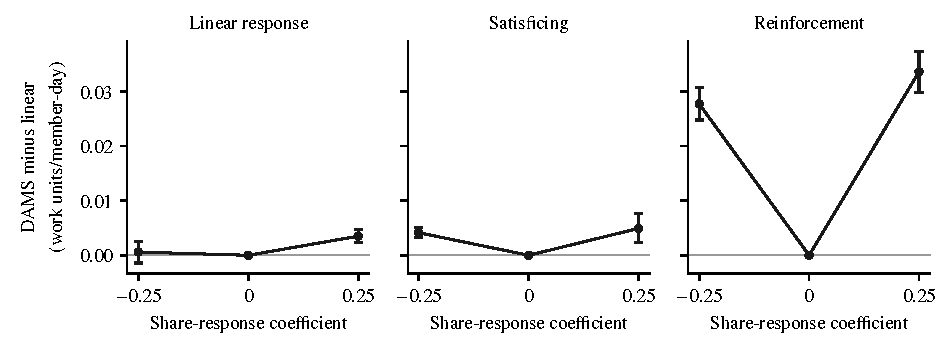
\includegraphics[width=\textwidth]{figures/results/response-boundaries.pdf}
\caption{Structural dependence of the DAMS--linear work contrast. Eight paired worlds per point; three effort rules and three predeclared response coefficients. Bars are descriptive 95\% Monte Carlo intervals conditional on each rule. Lines join sampled points without fitting. The zero channel is a mechanism null; negative responses provide an adverse case. Coefficients are unestimated design assumptions, not psychological measurements.}
\label{fig:response-boundaries}
\end{figure}
\begin{figure}[tbp]
\centering
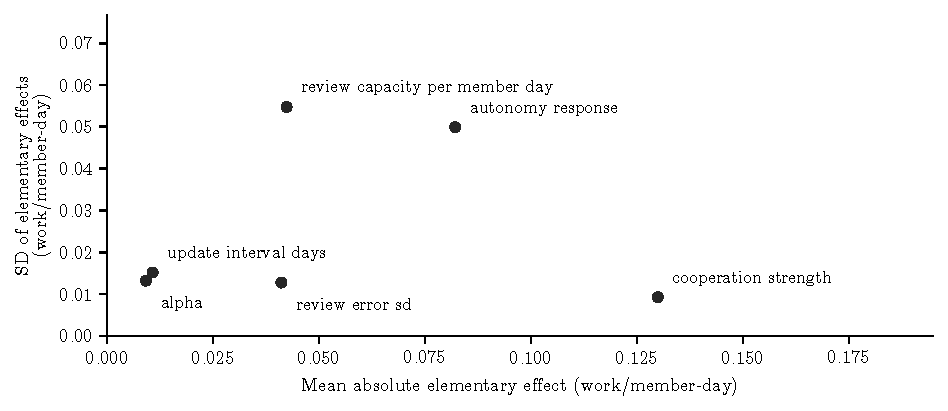
\includegraphics[width=\textwidth]{figures/results/sensitivity-screen.pdf}
\caption{Finite-difference screen over six independent design factors: eight randomized paths, three paired worlds at each step, four levels per factor. Horizontal position is mean absolute full-range elementary effect; vertical position is its path dispersion. This is a structural screening diagnostic, not Sobol indices or a probabilistic population variance decomposition. Input ranges and every path are retained in the repository.}
\label{fig:sensitivity-screen}
\end{figure}
\begin{table}[tbp]
\centering\small
\caption{DAMS--linear work contrasts across mechanistic stress contexts.}
\label{tab:context-results}
\begin{tabular}{lr}
\toprule
Synthetic context & Work difference [MC interval] \\
\midrule
noisy knowledge & 0.0034 [0.0028, 0.0041] \\
interdependent delivery & 0.0030 [0.0021, 0.0039] \\
distributed disruption & 0.0058 [0.0048, 0.0069] \\
high observation error & 0.0032 [0.0025, 0.0040] \\
cross principal confirmation & 0.0078 [0.0069, 0.0087] \\
review scarcity & 0.0100 [0.0091, 0.0110] \\
delayed accountability & 0.0023 [0.0016, 0.0031] \\
zero response & 0.0000 [0.0000, 0.0000] \\
reversed response & 0.0083 [0.0066, 0.0100] \\
\bottomrule
\end{tabular}
\par\smallskip\begin{minipage}{0.96\textwidth}\footnotesize Eight paired worlds per context, 120 members and 60 days. Intervals are descriptive 95\% normal Monte Carlo intervals; they do not include parameter or model uncertainty. Contexts change information, interdependence, site shocks, observation error, review resources, record assumptions, cadence or response. They are not calibrated industry, legal, demographic or sustainability cases.\end{minipage}
\end{table}
\begin{figure}[tbp]
\centering
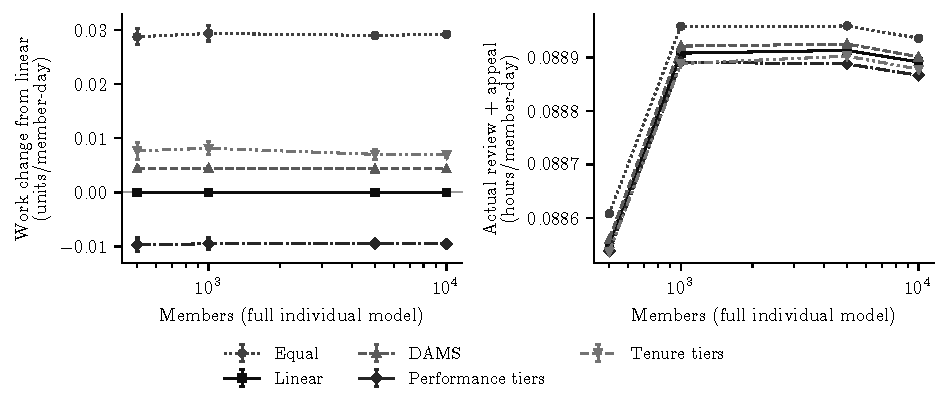
\includegraphics[width=\textwidth]{figures/results/organizational-scale.pdf}
\caption{Exploratory organizational scale comparisons: eight independent worlds at each of 500, 1,000, 5,000 and 10,000 full individual members, four guilds, two sites and 30 days. Left: paired work effect and descriptive 95\% Monte Carlo interval. Right: actual review and appeal service hours, excluding unused reservations and other unmodeled governance costs. Curves connect measured sizes, without extrapolating organizational benefits. Population growth also enlarges each fixed guild; guild count is not validator count.}
\label{fig:organizational-scale}
\end{figure}
\begin{figure}[tbp]
\centering
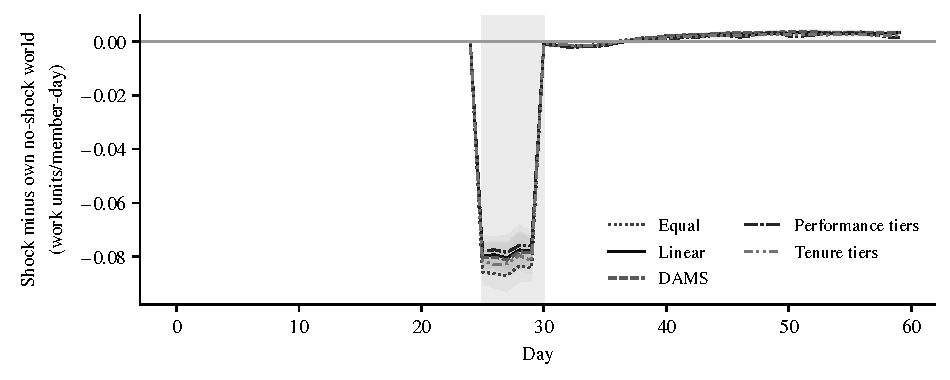
\includegraphics[width=\textwidth]{figures/results/shock-recovery.pdf}
\caption{Matched shock and no-shock output trajectories for five policies: eight independent world pairs per policy, 120 members and 60 days. Site 0 experiences a 0.7 output multiplier on days 25--29. Lines show paired mean work differences with pointwise descriptive 95\% Monte Carlo bands; zero is the matched no-shock outcome, not a pre-shock trend forecast. Repository recovery time is the first post-shock start of three days at least 99\% of own control output, with unrecovered worlds retained.}
\label{fig:shock-recovery}
\end{figure}
\begin{table}[tbp]
\centering\small
\caption{Synthetic parameter and behavioral-model recovery with held-out worlds.}
\label{tab:synthetic-recovery}
\begin{tabular}{lrrrrr}
\toprule
Generating rule & Response & Chosen rule & Chosen response & Capacity & Holdout loss \\
\midrule
Linear & 0.00 & Linear & 0.25 & 0.9 & 5.26 \\
Linear & 0.25 & Linear & 0.50 & 0.9 & 6.90 \\
Satisficing & 0.00 & Satisficing & 0.00 & 0.9 & 5.72 \\
Satisficing & 0.25 & Satisficing & 0.00 & 0.9 & 7.60 \\
Memory & 0.00 & Memory & 0.00 & 0.9 & 2.97 \\
Memory & 0.25 & Memory & 0.25 & 0.9 & 2.93 \\
\bottomrule
\end{tabular}
\par\smallskip\begin{minipage}{0.96\textwidth}\footnotesize Six synthetic generating conditions; eight observation-training worlds and eight disjoint candidate-prediction worlds, with four fresh worlds in each held-out set. Distance combines work, regret, queue stock and trust after declared standardization. Selection uses training only. It is a procedure diagnostic with a finite candidate grid, not external calibration or statistical identification in real firms.\end{minipage}
\end{table}
Exact grid parameters were recovered in 3 of 6 generating conditions and the effort-rule class in 6 of 6. Multiple settings within the declared diagnostic tolerance remain in the retained feasible sets; their multiplicity is part of the result. Output-only linear and sublinear worlds with zero share response are exactly observationally equivalent in the dedicated null check.
